\section{Task Modeling and System Design}

\subsection{Task Modeling}

Wildfire rescue is a closed-loop decision task rather than an isolated
perception or allocation problem. In an operational mission, aerial observations
first reveal dispersed fire points; these points must then be organized into
actionable task zones. The fleet must allocate its limited energy,
payload, and flight time to these regions, while unexpected failures or changes
in the fire situation may require the current plan to be revised during
execution. We therefore abstract the real rescue workflow as a sequence from
fire-situation understanding to resource-constrained mission planning and
runtime replanning.

This workflow exposes three risks that organize the system design. First, a
generated mission plan can appear coherent while violating tactical or
structural constraints. Second, as resource and scheduling interactions become
more complex, one-shot reasoning may fail to use relevant experience from
previous missions. Third, a plan that is feasible initially can become obsolete
after the fire, fleet, or mission state changes. High-level closed-loop decision
making must therefore check candidate plans before execution, recover relevant
experience when operational pressure increases, and revise the active mission
after runtime perturbations. The task model below represents the information
needed to support this continuing decision loop.

For each mission, the rescue world is represented by the structured state
\[
S=\{O,F,R,U,C,E\}.
\]
Here, $O$ denotes aerial observations; $F$ denotes fire points; $R$ denotes
task zones; $U$ denotes UAV operational states; $C$ denotes mission constraints;
and $E$ denotes runtime perturbations. This representation
separates the underlying rescue world from the information available to the
decision system. At mission start, the system receives $X_0=\{O,U,C\}$,
whereas $F$ and $R$ must be inferred from the observation. When a runtime
perturbation occurs, it receives the updated operational state $U_t$ and the
observed perturbation $E_t$. The required outputs are an initial mission plan
$P$ and, when necessary, a revised plan $P'$.

The resulting task model comprises the following decision chain:
\[
\begin{gathered}
O \rightarrow F \rightarrow R,\qquad (R,U,C) \rightarrow P, \\
(P,U_t,E_t) \rightarrow P'.
\end{gathered}
\]
The first two relations transform raw aerial observations into an actionable
regional representation of the fire situation. The third relation generates an
executable fleet plan under operational constraints. The final relation adapts
that plan to changes encountered during execution. This formulation captures
the continuous rescue workflow while retaining the stage-specific information
needed to design and evaluate a closed-loop system.

\subsection{System Overview}

\begin{figure*}[!t]
    \centering
    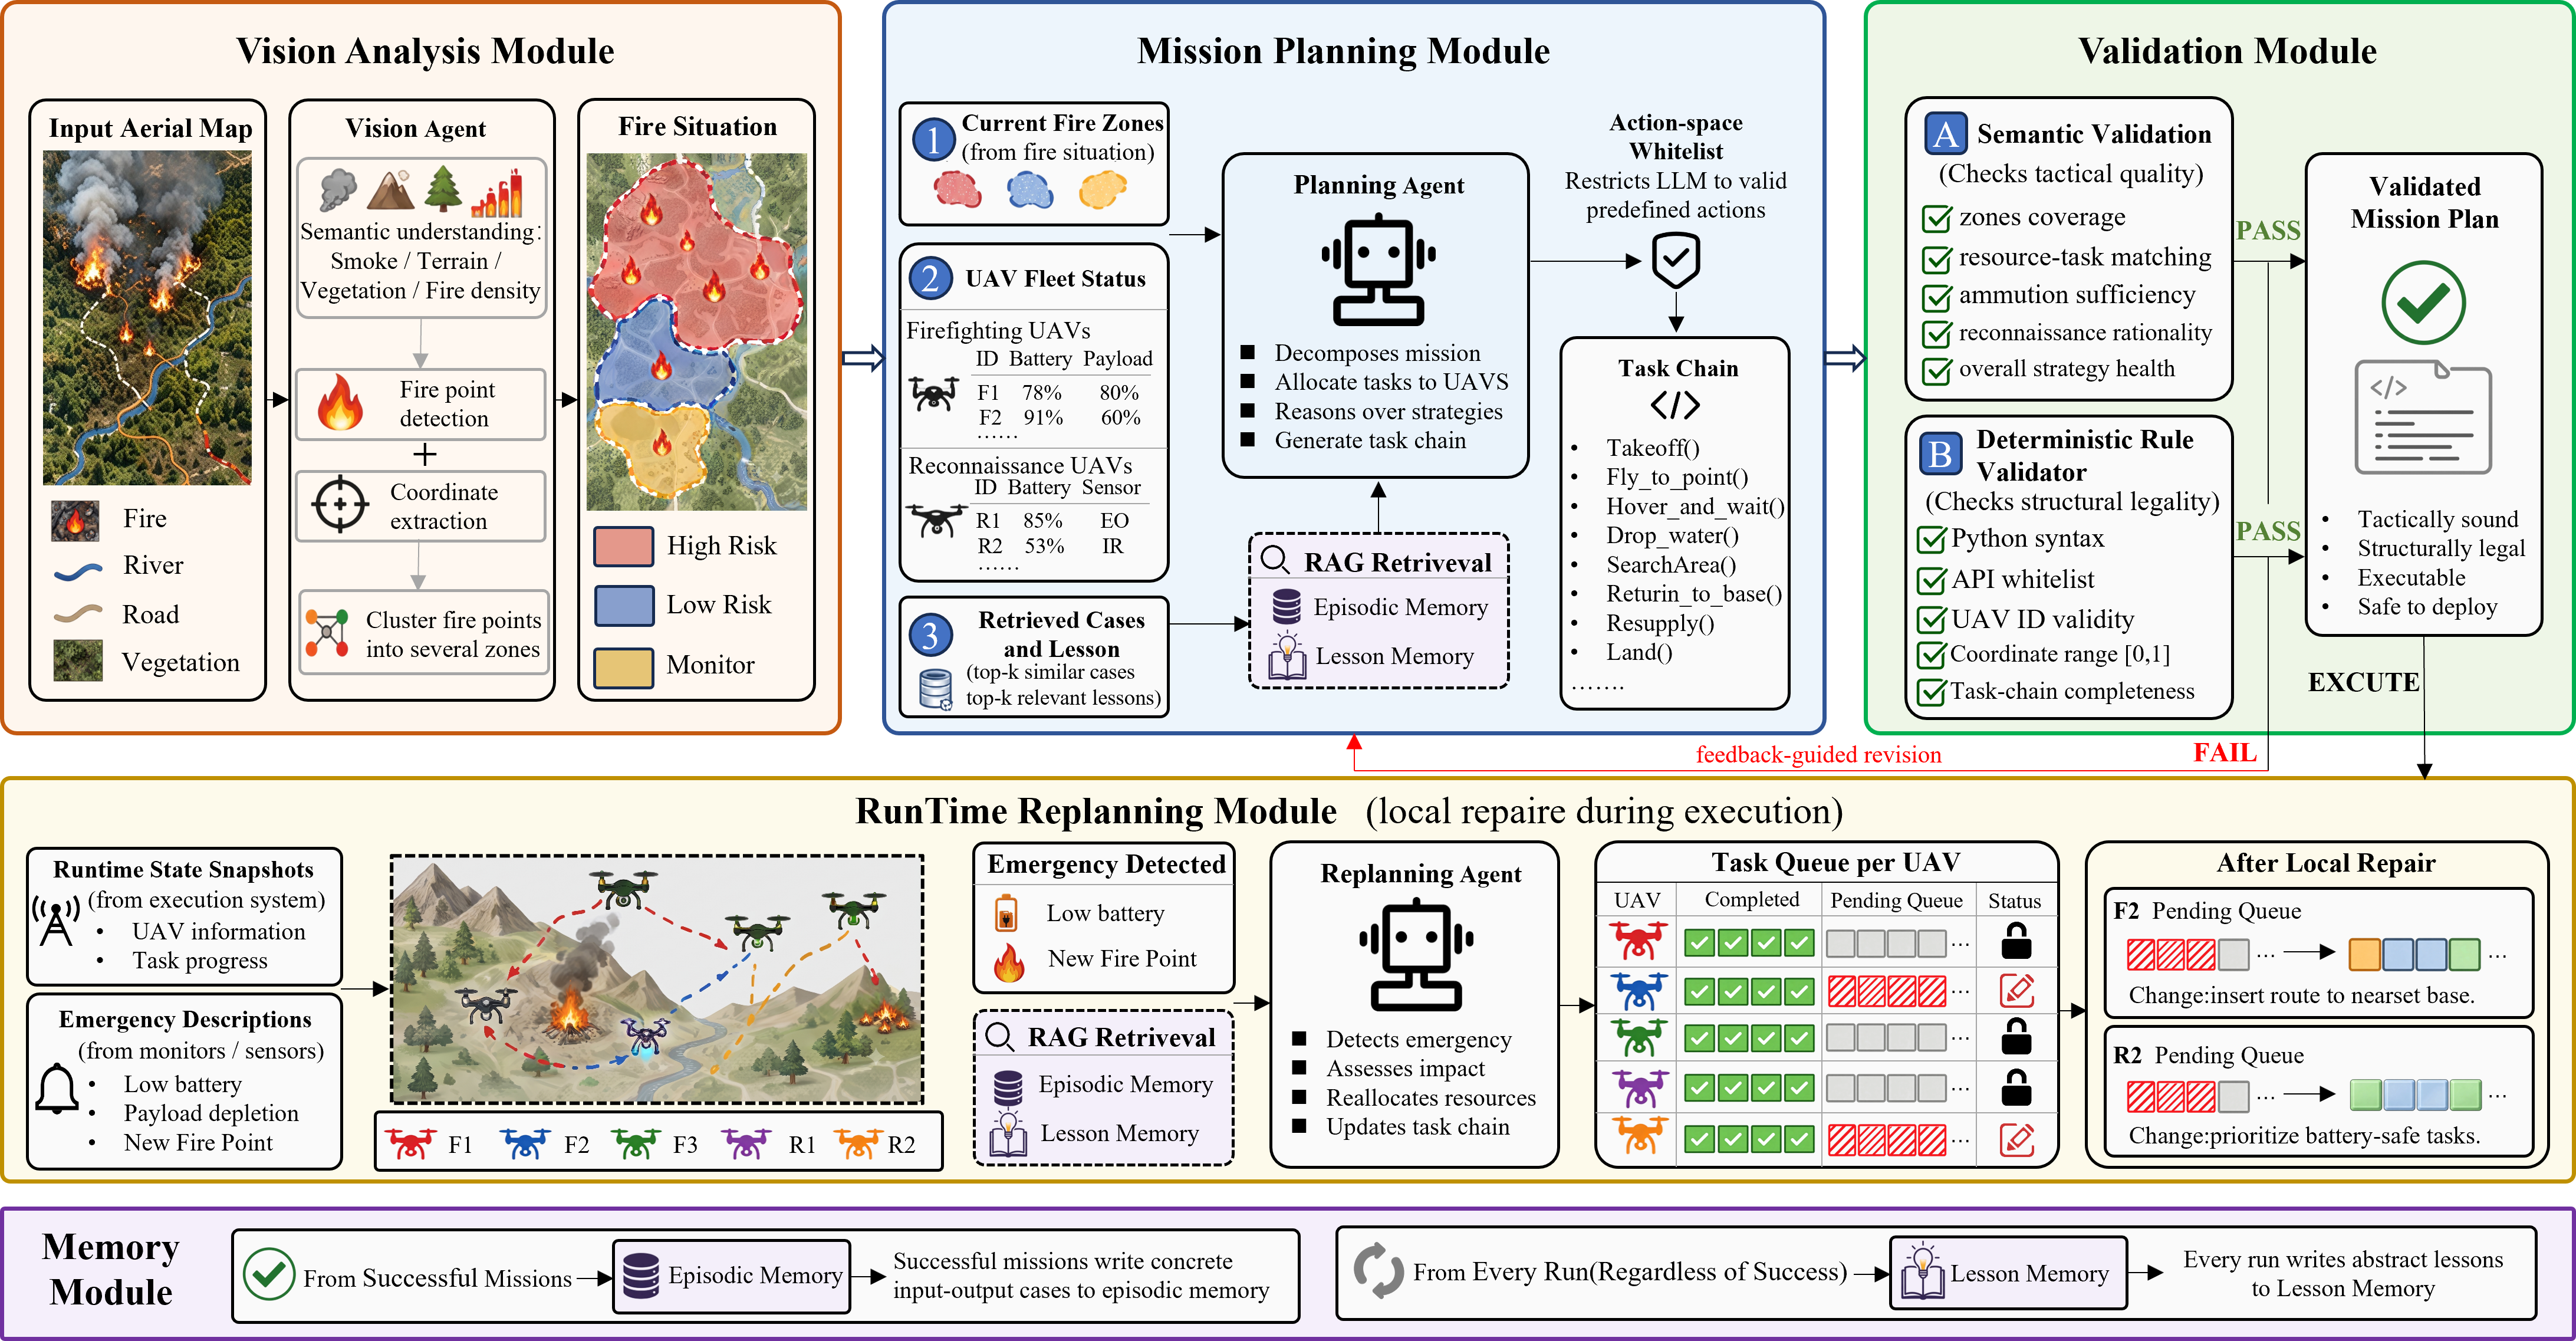
\includegraphics[width=1\textwidth]{figures/system-overview.png}
    \caption{Overview of the proposed system.}
    \label{fig:method-overview}
\end{figure*}

Based on the task model above, the proposed LLM-centered closed-loop decision
framework is organized around the flow of mission state, candidate plans,
corrective feedback, and prior experience.
Before execution, Vision Analysis transforms aerial fire imagery into fire
points and task zones. Mission Planning combines this representation with fleet
states, operational constraints, and retrieved experience from Memory to
produce a candidate plan. Validation then either accepts the plan or routes
targeted feedback back to Mission Planning for correction. This pre-execution
loop can repeat until an executable mission plan is accepted.

During execution, the accepted plan is evaluated against updated fleet states
and runtime perturbations. When an event invalidates part of the plan, Runtime
Replanning uses the current execution state and relevant Episodic Memory to
revise the affected part. Mission traces and outcomes are subsequently stored
as episodic cases or distilled into lessons by Memory. In this way,
Memory supports both initial planning and runtime replanning, while Validation
and execution feedback close the decision loop at different stages.
Figure~\ref{fig:method-overview} shows this information and feedback flow. 

\paragraph{Vision Analysis.} Vision Analysis anchors the decision loop by
reducing the ambiguity between raw aerial observations and the planning state.
It converts raw aerial imagery into a structured description of the fire
situation.
This module uses a multimodal LLM to perform two tasks in a single inference pass.
First, it detects all visible fire points in the image and outputs their normalized coordinates.
Second, it clusters these points by spatial density, partitioning the continuous fire field
into several discrete task zones.

This module uses a multimodal LLM rather than a vision-only model because zone division
depends on more than fire point locations.
The division also depends on visual context, such as smoke, vegetation,
and terrain boundaries.
These cues require joint reasoning over appearance and spatial semantics.
The resulting fire points and task zones provide the shared initial-state
representation used by Mission Planning.

\paragraph{Mission Planning.} Mission Planning addresses the fleet-level
coupling among task priorities, vehicle states, and resource constraints. It is
the core decision module and converts the structured fire situation produced by
Vision Analysis into a candidate multi-UAV collaborative plan. A planning LLM
generates a complete task chain for each UAV in the fleet, covering task
allocation, temporal sequencing, and endurance management. To keep outputs
controllable, the LLM is restricted to a predefined set of allowable actions.

Mission Planning combines the fire situation, retrieved experience,
and operational constraints.
It receives the structured fire situation from Vision Analysis,
retrieves relevant past cases and lessons from both memory modules,
and produces a coordinated plan in which each UAV's task chain respects
the fleet's capabilities and the mission's operational constraints.
Formally, the planning process is expressed as
\begin{equation}
P=\mathcal{G}\bigl(R,U,C,M_E(q),M_L(q)\bigr),
\qquad q=q(R,U,C),
\label{eq:memory-augmented-planning}
\end{equation}
where $\mathcal{G}$ denotes the planning LLM, $q$ is a query constructed from
the current task zones, fleet states, and constraints, and $M_E(q)$ and $M_L(q)$
denote the episodic cases and lessons retrieved for that query, respectively.
The resulting $P$ is a candidate plan rather than an automatically trusted
output; it is passed to Validation before mission execution.

\paragraph{Validation.} Validation addresses the risk that a linguistically
coherent candidate plan may still be tactically implausible or structurally
invalid. The module assesses each candidate plan through two sequential checks.
Together, the two checks form the audit--correction loop: when either one
rejects a plan, its feedback is routed back to Mission Planning for revision.
This loop turns validation failures into targeted feedback for the next
planning attempt.

The first check, Semantic Validation, uses an independent LLM to evaluate the plan
from a tactical rationality perspective. It examines zone coverage completeness,
resource-task matching, payload adequacy, and overall strategic health.
Using a separate LLM rather than asking the planning LLM to self-check
avoids self-consistency bias.

The second check, Deterministic Rule Validation, uses a rule engine to verify
structural legality, including UAV existence, coordinate validity, and task chain
completeness. Unlike the semantic check, this rule check asks whether the plan
is structurally legal.
This question can be answered deterministically within the defined rule set.
Only a plan accepted by both checks proceeds to execution, preserving the
separation between plan generation and plan acceptance.


\paragraph{Runtime Replanning.} Runtime Replanning addresses the risk that an
accepted plan becomes invalid after the operational state changes. This module
handles runtime perturbations during mission execution.
It takes a runtime state snapshot as input, including current positions, battery levels,
payloads, and task progress for each UAV.
Its output is not a new global plan, but a local revision of the current plan.
Unlike the main pipeline, Runtime Replanning reasons about a dynamic execution state and
changes only the affected part of the plan.

When a runtime perturbation occurs, the module retrieves similar fault cases
from Episodic Memory as repair references.
These cases describe how comparable failures were resolved in past missions,
providing the replanning LLM with tactical precedents for the current situation.
The resulting local revision closes the execution-feedback loop without
restarting the complete pre-execution pipeline.

\paragraph{Memory.} Memory addresses the risk that relevant prior experience is
unavailable when coupled resource, scheduling, or event conditions make the
current decision less routine. It allows the system to reuse past experience.
The two memory modules differ in what they store and how their contents are
used.

Episodic Memory stores concrete successful cases as input--output pairs.
Each case records the situation, the generated or revised plan,
and the corresponding outcome.
Cases are indexed by situational features, so that when a new mission situation arises,
the system retrieves the most similar past cases as tactical references.
Specifically, the episodic memory is represented as
\begin{equation}
M_E=\{(z_i,P_i,o_i)\}_{i=1}^{N_E},
\label{eq:episodic-memory}
\end{equation}
where $z_i$, $P_i$, and $o_i$ denote the task situation, the associated plan,
and the execution outcome of case $i$, respectively. For either episodic
memory or lesson memory, the system retrieves the $K$ most semantically similar
entries to the current query according to
\begin{equation}
\begin{aligned}
\mathcal{R}_K(q,M)
&=\underset{m_i\in M}{\operatorname{TopK}}\;
  \operatorname{sim}(q,m_i),\\
\operatorname{sim}(q,m_i)
&=\frac{\phi(q)^\top\phi(m_i)}
{\lVert\phi(q)\rVert_2\lVert\phi(m_i)\rVert_2}.
\end{aligned}
\label{eq:semantic-memory-retrieval}
\end{equation}
where $M\in\{M_E,M_L\}$ is the queried memory, $\phi(\cdot)$ maps a query
or memory entry to its semantic embedding, and $\operatorname{sim}(\cdot,\cdot)$
is the cosine similarity. The retrieved set is supplied to the corresponding
planning or replanning prompt as reference information.

Lesson Memory serves a different role. Instead of storing concrete cases,
it keeps higher-level lessons distilled from every run.
After each mission, an LLM reviews the full execution trace.
The trace includes the initial plan, validation feedback, runtime perturbations,
replanning actions, and final scores.
The LLM then extracts concise, reusable lessons.
These lessons capture patterns such as common planning mistakes, resource estimation biases,
and effective repair strategies.
Together, the two forms of Memory connect prior outcomes to current decisions:
Episodic Memory supplies concrete tactical precedents, whereas Lesson Memory
supplies reusable guidance about recurring planning and resource-management
patterns.

\endinput
